%%
% このファイルは、筑波大学情報学群情報科学類の
% 卒業研究中間報告用本体のサンプルです。
% このファイルを書き換えて、この例と同じような書式の論文本体を
% LaTeXを使って作成することができます。
% 
% PC環境や、LaTeX環境の設定によっては漢字コードや改行コードを
% 変更する必要があります。
%%
\documentclass[a4paper,10pt]{jarticle}

%%【PDF, JPEG, PNG等の画像の貼り込み】
%% 利用するパッケージを選んで下さい。
\usepackage[dvipdfmx]{graphicx} % for \includegraphics[width=3cm]{sample.pdf}
%\usepackage{epsfig} % for \psfig{file=sample.eps,width=3cm}
%\usepackage{epsf} % for \epsfile{file=sample.eps,scale=0.6}
%\usepackage{epsbox} % for \epsfile{file=sample.eps,scale=0.6}

\usepackage{times} % use Times Font instead of Computer Modern
% \usepackage{luatexja-fontspec}
% \setmainfont[Ligatures=TeX]{Times New Roman}
% \setmainjfont[BoldFont=MS Gothic]{MS Mincho}
\usepackage{url}

\setcounter{tocdepth}{3}
\setcounter{page}{1}

\setlength{\oddsidemargin}{-.1in}
\setlength{\evensidemargin}{-.1in}
\setlength{\topmargin}{-4em}
\setlength{\textwidth}{6.5in}
\setlength{\textheight}{10in}
\setlength{\parskip}{0em}
\setlength{\topsep}{0em}
\setlength{\columnsep}{3zw}

%% タイトル生成用パッケージ(重要)
\usepackage{coins-jp}

%% タイトル
\title{並列ファイルシステムのための効率的なシステムコールフックライブラリの設計と評価}
%% 著者
\gakuseki{202111759}
\author{宮内遥楓}
%% 指導教員
\advisor{建部修見}

%% 年度と主専攻名
%% 必要に応じて書き替えて下さい。
\fiscalyear{2024}
%\majorfield{ソフトウェアサイエンス主専攻}
\majorfield{情報システム主専攻}
%\majorfield{知能情報メディア主専攻}

%% 提出日
\year{2024}
\month{10}
\day{24}

\begin{document}

\maketitle

\section{序論}

ユーザー空間並列ファイルシステムは、ストレージシステムの性能を向上させるために開発されてきた~\cite{tatebe2022chfs, 8514892, 10177390}。 
一方、POSIXインターフェースは、標準として長い間アプリケーションに使用されてきた。 
多くのアプリケーションを動作させるためにはPOSIXインタフェースのサポートが必要であるが、
FUSEやシステムコールインターセプションライブラリなどの既存の手法には様々な問題がある。
本研究では、バイナリ書き換えに基づくシステムコールフック機構であるzpoline~\cite{288689}を利用することでこの問題を解決し、
その性能結果を示す。

\section{既存手法}

\subsection{FUSE}
FUSE(Filesystem in Userspace)は、ユーザ空間ファイルシステムを実装するのに広く用いられている。 
FUSEはユーザー空間でPOSIXインターフェースを完全にサポートできるが、オーバーヘッドが大きい。


\subsection{システムコールインターセプトライブラリ}
gotcha~\cite{gotcha}のようなシステムコールインターセプトライブラリは、libc(C標準ライブラリ)の関数呼び出しをインターセプトする。
libc(C標準ライブラリ)の関数と同じ名前の関数を定義し、LD\_PRELOADを使うことで、システムコールインターセプトライブラリで定義した関数が呼び出される。
しかしながら、libcの関数はシステムコールに対応していないので全てのシステムコールをフックすることができない、libc内でマクロを
利用して呼び出されたシステムコールをフックできないなどの問題がある。


\section{設計}
本研究では、並列ファイルシステムの1つであるCHFSを対象にシステムコールフックライブラリを設計・実装する。
提案するシステムコールフックライブラリは、zpolineを用い、read、write、open、close、stat、lstat、lseek、pread64、pwrite64、
openat、fsync、newfstatシステムコールをフックする。ファイルにアクセスした際、パス名が仮想マウントポイント/chfsの下にある場合、
CHFSのクライアントライブラリを呼び出し、そうでない場合は元のシステムコールを呼び出す。

\section{評価}
本研究では、zpolineを用いたシステムコールフックライブラリの性能を、CHFSのAPIを直接呼び出した場合やFUSEを使用した場合と比較して評価した。
Pegasusスーパーコンピュータ上でCHFSクライアントに1ノード、CHFSサーバーに10ノード使用し、各ノードは200Gbpsの
InfiniBand NDR200で接続されている。計測にはIORベンチマークを使用する。

  \begin{figure}[h]
	\centering
	\begin{minipage}[b]{0.49\columnwidth}
		\centering
		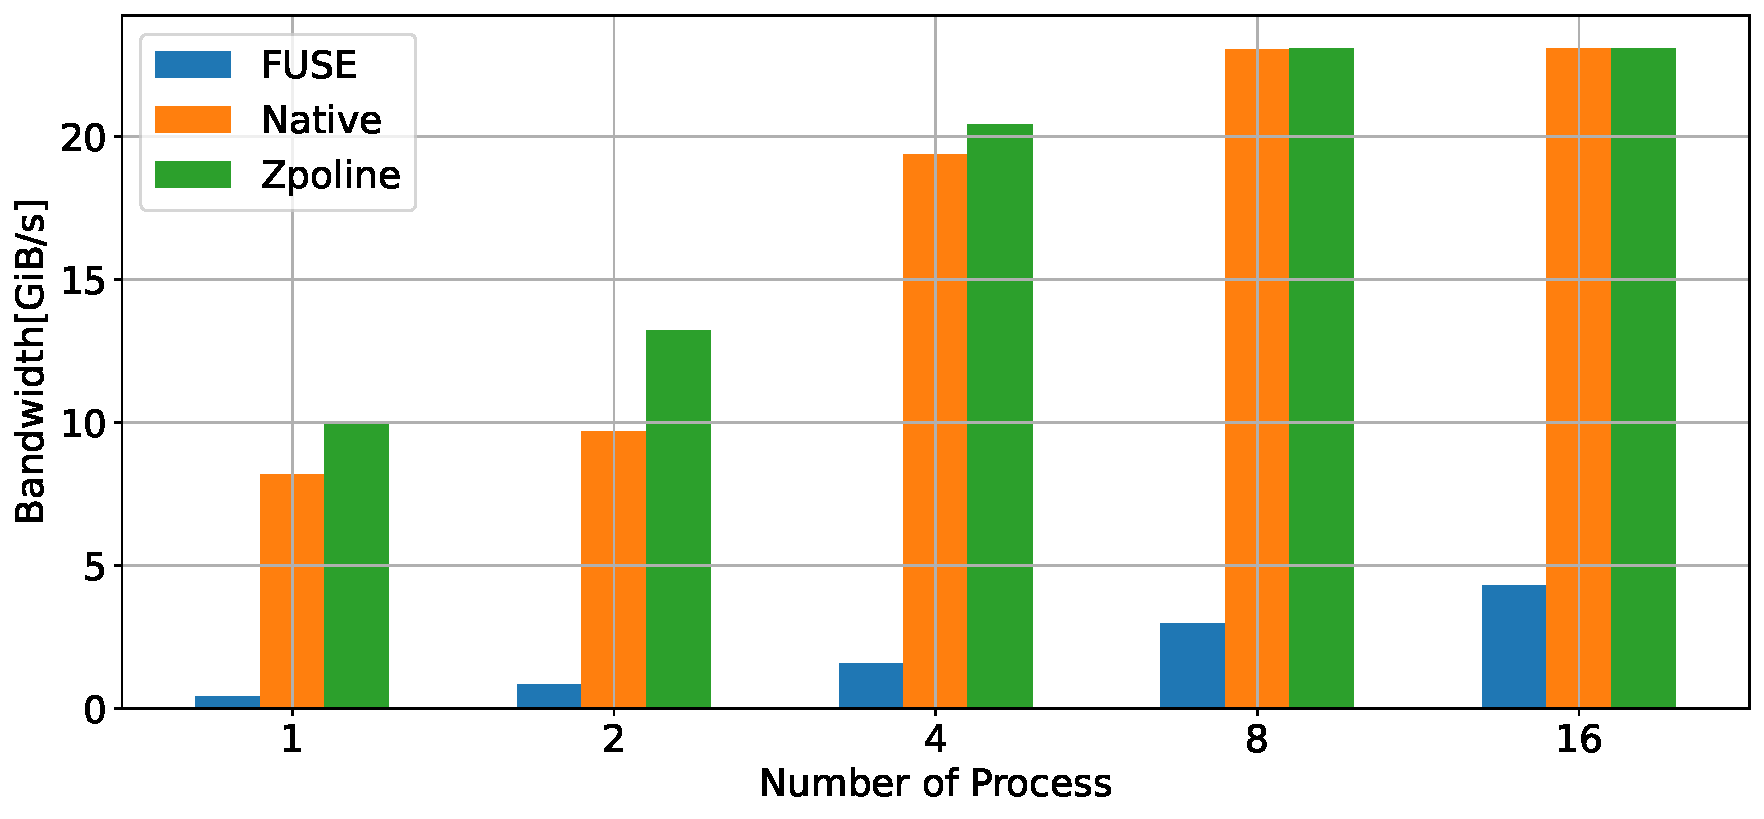
\includegraphics[width=0.9\linewidth]{./ior_benchmark_read.pdf}
		\caption{IOR file-per-process 読込み性能}
		\label{fig:Evaluation read}
	\end{minipage}
	\begin{minipage}[b]{0.49\columnwidth}
		\centering
		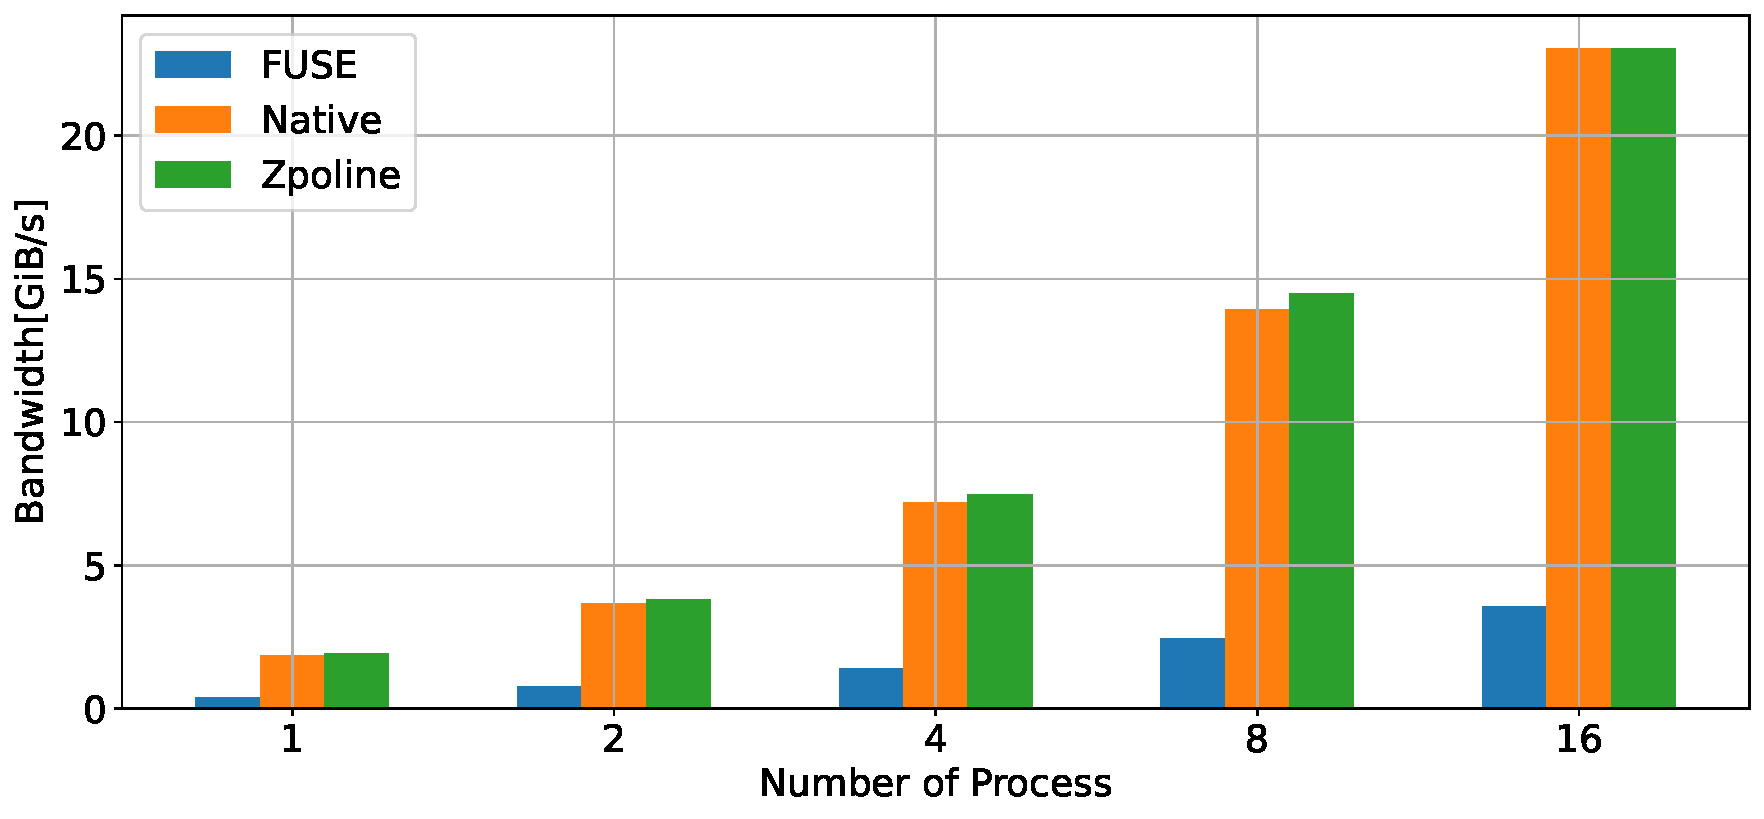
\includegraphics[width=0.9\linewidth]{./ior_benchmark_write.pdf}
		\caption{IOR file-per-process 書込み性能}
		\label{fig:Evaluation write}
	\end{minipage}
	\end{figure}

\figurename~\ref{fig:Evaluation read}で読込み性能を、\figurename~\ref{fig:Evaluation write}で書込み性能を示す。
zpolineを使用したシステムコールフックライブラリは、CHFSのAPIを直接呼び出した場合と同等の性能を示した。
またFUSEを使用した場合と比較してより高い性能を示し、特に16プロセスにおいてFUSEの5.3倍高い読込み性能、
6.4倍高い書込み性能を示した。

\section{結論}
ユーザー空間におけるPOSIXインターフェースのサポートにはいくつかの問題があったが、本研究により、zpolineを使用することで
これらの問題を解決できることが示された。提案したシステムコールフックライブラリはCHFSのAPIを直接呼び出した場合と同等の性能を示し、
FUSEの5.3倍から6.4倍の性能結果を示した。

\bibliography{main}
\bibliographystyle{junsrt}

\end{document}
